\chapter{Sets}

\section{Basic notions}

\begin{definition}
A \emph{set} is a collection of objects, called its \emph{elements}. We write $x \in S$ if $x$
is an element of $S$ and $x \notin S$ otherwise. The \emph{empty set} $\emptyset$ has no
elements. A set with finitely many elements is finite; its number of elements is its
\emph{cardinality}, $\abs{S}$.
\end{definition}

Sets are described either by listing, $\{1,2,3\}$, or with \emph{set-builder notation}
$\{x \in U : P(x)\}$, ``the set of $x$ in $U$ such that $P(x)$''. Order and repetition do not
matter: $\{1,2,2,3\} = \{3,1,2\}$.

\begin{example}
\begin{itemize}
  \item $\{n \in \Z : n^2 < 10\} = \{-3,-2,-1,0,1,2,3\}$.
  \item $\{2k + 1 : k \in \Z\}$ is the set of odd integers.
  \item $\{\emptyset\} \ne \emptyset$: the former has one element.
  \item $\abs{\{1,\{1,2\},\emptyset\}} = 3$.
\end{itemize}
\end{example}

\section{Set operations}

Let $A,B$ be subsets of a universal set $U$.

\begin{definition}
\begin{itemize}
  \item Union: $A \cup B = \{x : x \in A \vee x \in B\}$.
  \item Intersection: $A \cap B = \{x : x \in A \wedge x \in B\}$.
  \item Difference: $A - B = A \setminus B = \{x : x \in A \wedge x \notin B\}$.
  \item Complement: $\bar A = A^c = \{x \in U : x \notin A\}$.
\end{itemize}
$A$ and $B$ are \emph{disjoint} if $A \cap B = \emptyset$.
\end{definition}

The shaded regions below show each operation.

\begin{center}
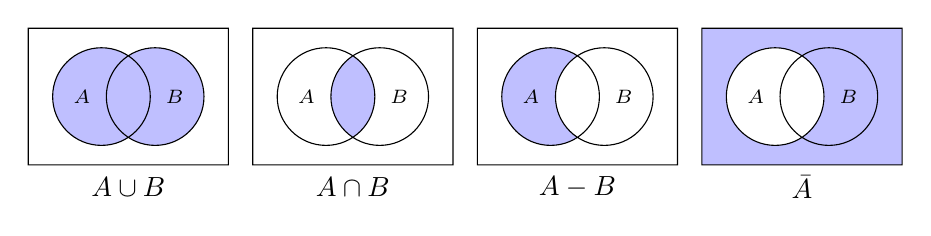
\begin{tikzpicture}[scale=0.62]
  \def\A{(0,0) circle (1)}
  \def\B{(1.1,0) circle (1)}
  \def\U{(-1.5,-1.4) rectangle (2.6,1.4)}
  % union
  \begin{scope}
    \fill[blue!25] \A; \fill[blue!25] \B;
    \draw \U \A \B; \node at (0.55,-1.85) {$A \cup B$};
    \node at (-0.4,0) {\scriptsize $A$}; \node at (1.5,0) {\scriptsize $B$};
  \end{scope}
  % intersection
  \begin{scope}[xshift=4.6cm]
    \begin{scope} \clip \A; \fill[blue!25] \B; \end{scope}
    \draw \U \A \B; \node at (0.55,-1.85) {$A \cap B$};
    \node at (-0.4,0) {\scriptsize $A$}; \node at (1.5,0) {\scriptsize $B$};
  \end{scope}
  % difference
  \begin{scope}[xshift=9.2cm]
    \fill[blue!25] \A; \fill[white] \B;
    \draw \U \A \B; \node at (0.55,-1.85) {$A - B$};
    \node at (-0.4,0) {\scriptsize $A$}; \node at (1.5,0) {\scriptsize $B$};
  \end{scope}
  % complement
  \begin{scope}[xshift=13.8cm]
    \fill[blue!25] \U; \fill[white] \A;
    \draw \U \A \B; \node at (0.55,-1.85) {$\bar A$};
    \node at (-0.4,0) {\scriptsize $A$}; \node at (1.5,0) {\scriptsize $B$};
  \end{scope}
\end{tikzpicture}
\end{center}

The definitions translate set operations into the logical connectives of Chapter 1:
$\cup$ is $\vee$, $\cap$ is $\wedge$, complement is $\neg$. Consequently set identities
mirror logical equivalences.

\begin{example}
Let $U = \{1,\dots,10\}$, $A = \{1,2,3,4,5\}$, $B = \{2,4,6,8,10\}$. Then
$A \cup B = \{1,2,3,4,5,6,8,10\}$, $A \cap B = \{2,4\}$, $A - B = \{1,3,5\}$,
$\bar B = \{1,3,5,7,9\}$.
\end{example}

Placing each element of $U$ in its region of the Venn diagram makes all four answers visible
at once:
\begin{center}
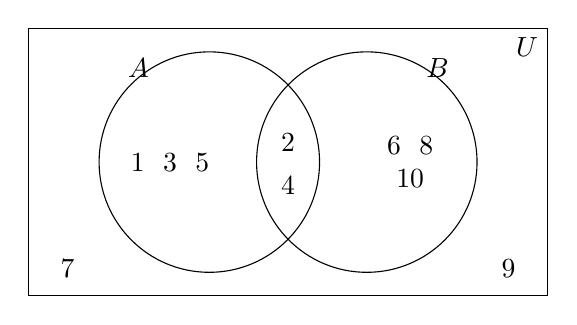
\begin{tikzpicture}
  \draw (-2.3,-1.7) rectangle (4.3,1.7);
  \node[below left] at (4.3,1.7) {$U$};
  \draw (0,0) circle (1.4) (2,0) circle (1.4);
  \node at (-0.9,1.2) {$A$}; \node at (2.9,1.2) {$B$};
  \node at (-0.5,0) {$1\ \ 3\ \ 5$};
  \node at (1,0.25) {$2$}; \node at (1,-0.3) {$4$};
  \node[align=center] at (2.55,0) {$6\ \ 8$\\$10$};
  \node at (-1.8,-1.35) {$7$}; \node at (3.8,-1.35) {$9$};
\end{tikzpicture}
\end{center}

\begin{theorem}[De Morgan's laws for sets]
$\overline{A \cup B} = \bar A \cap \bar B$ and $\overline{A \cap B} = \bar A \cup \bar B$.
\end{theorem}

\begin{aside}
Venn diagrams are useful for guessing whether an identity is true, but are not accepted as a
proof.
\end{aside}

\begin{center}
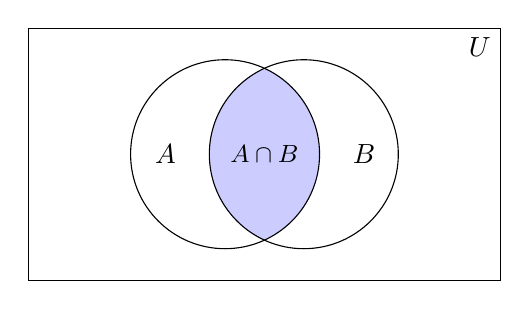
\begin{tikzpicture}
  \draw (-2.5,-1.6) rectangle (3.5,1.6) node[below left] {$U$};
  \begin{scope}
    \clip (0,0) circle (1.2);
    \fill[blue!20] (1,0) circle (1.2);
  \end{scope}
  \draw (0,0) circle (1.2) node[left=0.5cm] {$A$};
  \draw (1,0) circle (1.2) node[right=0.5cm] {$B$};
  \node at (0.5,0) {\small $A\cap B$};
\end{tikzpicture}
\end{center}

\section{Subsets and set equality}

\begin{definition}
$A$ is a \emph{subset} of $B$, $A \subseteq B$, if every element of $A$ is an element of $B$:
$\forall x,\ x \in A \Rightarrow x \in B$. $A$ is a \emph{proper subset}, $A \subsetneq B$, if
additionally $A \ne B$. Two sets are \emph{equal} if $A \subseteq B$ and $B \subseteq A$.
\end{definition}

\begin{important}[Templates]
\begin{itemize}
  \item To show $A \subseteq B$: ``Let $x \in A$. \dots\ Therefore $x \in B$.''
  \item To show $A = B$: show $A \subseteq B$ and $B \subseteq A$ (two ``element chasing''
        arguments), or a chain of equivalences $x \in A \iff \cdots \iff x \in B$.
  \item To show $A \not\subseteq B$: find one $x \in A$ with $x \notin B$.
\end{itemize}
\end{important}

Note $\emptyset \subseteq A$ for every set $A$ (vacuously), and $\in$ is not the same as
$\subseteq$: $1 \in \{1,2\}$ but $\{1\} \subseteq \{1,2\}$.

\begin{example}
Show $\{n \in \Z : 6 \mid n\} \subseteq \{n \in \Z : 2 \mid n\}$.
Let $n$ be in the first set, so $n = 6k$ for some $k \in \Z$. Then $n = 2(3k)$, so $2 \mid n$
and $n$ is in the second set. The reverse inclusion fails: $2$ is in the second set but not
the first.
\end{example}

\begin{proposition}
For sets $A,B,C$: $A \cap (B \cup C) = (A \cap B) \cup (A \cap C)$.
\end{proposition}
\begin{proof}
($\subseteq$) Let $x \in A \cap (B\cup C)$. Then $x \in A$ and ($x \in B$ or $x \in C$).
If $x \in B$ then $x \in A \cap B$; if $x \in C$ then $x \in A\cap C$. Either way
$x \in (A\cap B)\cup(A\cap C)$.

($\supseteq$) Let $x \in (A\cap B)\cup(A \cap C)$. If $x \in A\cap B$, then $x \in A$ and
$x \in B \subseteq B \cup C$. If $x \in A \cap C$, then $x \in A$ and $x \in C \subseteq B\cup C$.
In both cases $x \in A \cap (B \cup C)$.
\end{proof}

The two sides of the distributive law shade the same region (a Venn diagram suggests the
identity; the element-chasing proof above establishes it):
\begin{center}
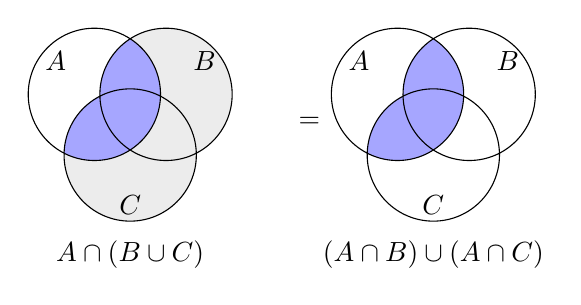
\begin{tikzpicture}[scale=0.7]
  \def\A{(0,0) circle (1.2)}
  \def\B{(1.3,0) circle (1.2)}
  \def\C{(0.65,-1.1) circle (1.2)}
  \begin{scope}
    \fill[gray!15] \B; \fill[gray!15] \C;
    \begin{scope} \clip \A; \fill[blue!35] \B; \fill[blue!35] \C; \end{scope}
    \draw \A \B \C;
    \node at (-0.7,0.6) {$A$}; \node at (2.0,0.6) {$B$}; \node at (0.65,-2.0) {$C$};
    \node at (0.65,-2.9) {$A \cap (B \cup C)$};
  \end{scope}
  \node at (3.9,-0.5) {$=$};
  \begin{scope}[xshift=5.5cm]
    \begin{scope} \clip \A; \fill[blue!35] \B; \end{scope}
    \begin{scope} \clip \A; \fill[blue!35] \C; \end{scope}
    \draw \A \B \C;
    \node at (-0.7,0.6) {$A$}; \node at (2.0,0.6) {$B$}; \node at (0.65,-2.0) {$C$};
    \node at (0.65,-2.9) {$(A \cap B) \cup (A \cap C)$};
  \end{scope}
\end{tikzpicture}
\end{center}
(On the left, the light grey region is $B \cup C$.)

\begin{proposition}
$A \subseteq B$ if and only if $A \cap B = A$.
\end{proposition}
\begin{proof}
($\Rightarrow$) Assume $A \subseteq B$. Always $A \cap B \subseteq A$. Conversely if $x \in A$
then $x \in B$ by assumption, so $x \in A \cap B$. Hence $A \cap B = A$.
($\Leftarrow$) Assume $A \cap B = A$ and let $x \in A$. Then $x \in A \cap B$, so $x \in B$.
\end{proof}

\begin{example}[A non-obvious equality]
Let $S$ be the set of integers leaving remainder $1$ or $3$ when divided by $4$, and $T$ the
odd integers. Then $S = T$: if $n = 4k+1$ or $4k+3$ then $n = 2(2k) + 1$ or
$2(2k+1) + 1$, odd. Conversely if $n = 2m + 1$, then $m$ is even ($m = 2k$, $n = 4k+1$) or odd
($m = 2k+1$, $n = 4k+3$).
\end{example}

\begin{example}[Disproving an identity]
Is $A - (B - C) = (A - B) - C$? Try $A = B = C = \{1\}$: $A - (B-C) = \{1\} - \emptyset
= \{1\}$, while $(A - B) - C = \emptyset - \{1\} = \emptyset$. So the identity is false.
\end{example}

\section{Cartesian products and power sets}

\begin{definition}
The \emph{Cartesian product} of $A$ and $B$ is the set of ordered pairs
\[ A \times B = \{(a,b) : a \in A,\ b \in B\}. \]
Ordered pairs satisfy $(a,b) = (c,d) \iff a = c \text{ and } b = d$. If $A$ and $B$ are finite
then $\abs{A\times B} = \abs A\abs B$.
\end{definition}

\begin{example}
$\{1,2\} \times \{x,y,z\} = \{(1,x),(1,y),(1,z),(2,x),(2,y),(2,z)\}$, which has $2\cdot 3 = 6$
elements. Note $A \times B \ne B\times A$ in general. $\R \times \R = \R^2$ is the plane.
\end{example}

Drawing $A$ along one axis and $B$ along the other shows $A \times B$ as a grid of
$\abs A \cdot \abs B$ points:
\begin{center}
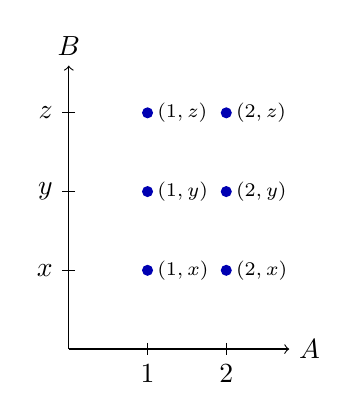
\begin{tikzpicture}
  \draw[->] (0,0) -- (2.8,0) node[right] {$A$};
  \draw[->] (0,0) -- (0,3.6) node[above] {$B$};
  \foreach \a in {1,2} { \draw (\a,0.08) -- (\a,-0.08) node[below] {$\a$}; }
  \foreach \b/\y in {x/1,y/2,z/3} {
    \draw (0.08,\y) -- (-0.08,\y) node[left] {$\b$};
    \foreach \a in {1,2} {
      \fill[blue!70!black] (\a,\y) circle (2pt);
      \node[right,font=\scriptsize] at (\a,\y) {$(\a,\b)$};
    }
  }
\end{tikzpicture}
\end{center}

\begin{proposition}
$A \times (B \cap C) = (A \times B) \cap (A \times C)$.
\end{proposition}
\begin{proof}
For any pair $(x,y)$:
\begin{align*}
(x,y) \in A\times(B\cap C) &\iff x \in A \wedge (y \in B \wedge y \in C)\\
&\iff (x \in A \wedge y \in B)\wedge(x \in A \wedge y \in C)\\
&\iff (x,y) \in (A\times B)\cap(A \times C).
\end{align*}
Every element of either side is an ordered pair, so the sets are equal.
\end{proof}

\begin{definition}
The \emph{power set} $\mathcal{P}(A)$ is the set of all subsets of $A$. If $\abs A = n$ then
$\abs{\mathcal P(A)} = 2^n$ (each element is either in or out of a subset).
\end{definition}

\begin{example}
$\mathcal P(\{1,2\}) = \{\emptyset,\{1\},\{2\},\{1,2\}\}$.
\end{example}

\section{Common pitfalls}
\begin{itemize}
  \item Confusing $\in$ with $\subseteq$, or $\emptyset$ with $\{\emptyset\}$.
  \item Proving only one inclusion when asked for equality.
  \item Starting an inclusion proof with a specific element instead of an arbitrary one.
  \item Using a Venn diagram as the proof.
\end{itemize}

\section{Summary}
\begin{itemize}
  \item Union, intersection, complement correspond to $\vee$, $\wedge$, $\neg$; set identities
        follow from logical equivalences.
  \item $A \subseteq B$: let $x \in A$ and show $x \in B$. $A = B$: show both inclusions.
  \item $A \times B$ is the set of ordered pairs; $\abs{A\times B} = \abs A\abs B$;
        $\abs{\mathcal P(A)} = 2^{\abs A}$.
\end{itemize}
